\section{Properties of random variables}

\subsection{a}
\subsubsection{i}
The definition of the expected value for a continuous random variable is:

$$\mathbb{E}[x] = \int_{-\infty}^{\infty} x f(x) dx$$

Where f(x) is the probability density function (pdf) of x. For a Gaussian random variable, the pdf is given by:

$$f(x) = \frac{1}{\sigma\sqrt{2\pi}} e^{-\frac{(x-\mu)^2}{2\sigma^2}}$$

Now, we need to compute the expected value:

$$\mathbb{E}[x] = \int_{-\infty}^{\infty} x \frac{1}{\sigma\sqrt{2\pi}} e^{-\frac{(x-\mu)^2}{2\sigma^2}} dx$$

Let's perform the substitution:

$$t = \frac{x-\mu}{\sqrt{2}\sigma}$$

Then,

$$x = \mu + \sqrt{2}\sigma t$$
$$dx = \sqrt{2}\sigma dt$$

Now, substitute these values into the expected value integral:

$$\mathbb{E}[x] = \frac{1}{\sigma\sqrt{2\pi}} \int_{-\infty}^{\infty} (\mu + \sqrt{2}\sigma t) e^{-t^2} (\sqrt{2}\sigma dt) = \frac{1}{\sqrt{\pi}} \int_{-\infty}^{\infty} (\mu + \sqrt{2}\sigma t) e^{-t^2} dt$$

Now, split the integral into two parts:

$$\mathbb{E}[x] = \frac{\mu}{\sqrt{\pi}} \int_{-\infty}^{\infty} e^{-t^2} dt + \frac{\sqrt{2}\sigma}{\sqrt{\pi}} \int_{-\infty}^{\infty} te^{-t^2} dt$$

Using the hint provided, we know that:

$$\int_{-\infty}^{\infty} e^{-t^2} dt = \sqrt{\pi}$$

The second integral is an odd function, and the integral over the whole real line of an odd function is zero. Therefore:

$$\int_{-\infty}^{\infty} te^{-t^2} dt = 0$$

Thus, the expected value is:$\mathbb{E}[x] = \mu + 0 = \mu$, which proves the question i).

\subsubsection{ii}

Using the definition of expected value:

$$Var[x] = \int_{-\infty}^{\infty} (x-\mu)^2 f(x) dx$$

Substitute the Gaussian pdf:

$$Var[x] = \int_{-\infty}^{\infty} (x-\mu)^2 \frac{1}{\sigma\sqrt{2\pi}} e^{-\frac{(x-\mu)^2}{2\sigma^2}} dx$$

Use the same substitution as before:

$$t = \frac{x-\mu}{\sqrt{2}\sigma}$$

$$x = \mu + \sqrt{2}\sigma t$$
$$dx = \sqrt{2}\sigma dt$$

Substitute these values into the integral:

$$Var[x] = \frac{1}{\sigma\sqrt{2\pi}} \int_{-\infty}^{\infty} (x-\mu)^2 e^{-\frac{(x-\mu)^2}{2\sigma^2}} dx$$

Substitute the values we found earlier:

$$Var[x] = \frac{1}{\sigma\sqrt{2\pi}} \int_{-\infty}^{\infty} (\sqrt{2}\sigma t)^2 e^{-t^2} (\sqrt{2}\sigma dt)$$

Simplify the expression:

$$Var[x] = \frac{2\sigma^2}{\sqrt{\pi}} \int_{-\infty}^{\infty} t^2 e^{-t^2} dt$$

To integrate the function $\int_{-\infty}^{\infty} t^2 e^{-t^2} dt$, let $u=t^2$, so that $du/dt=2t$ and $dt=du/2t$. Then, we can rewrite the integral as follows:

$$\int_{-\infty}^{\infty} t^2 e^{-t^2} dt=\int_{-\infty}^{\infty} \frac{1}{2}u e^{-u} \frac{du}{\sqrt{u}}$$

Next, we can use the gamma function, $\Gamma(n)=\int_{0}^{\infty} x^{n-1}e^{-x}dx$, to simplify the integral:

$$\int_{-\infty}^{\infty} t^2 e^{-t^2} dt=\int_{0}^{\infty} \frac{1}{2}u e^{-u} \frac{du}{\sqrt{u}}+\int_{-\infty}^{0} \frac{1}{2}u e^{-u} \frac{du}{\sqrt{u}}$$

$$=\frac{1}{2}\int_{0}^{\infty} u^{1/2-1}e^{-u}du+\frac{1}{2}\int_{0}^{\infty} (-u)^{1/2-1}e^{u}du$$

Using the definition of the gamma function, we can simplify the two integrals to obtain:

$$\int_{-\infty}^{\infty} t^2 e^{-t^2} dt=\frac{1}{2}\Gamma\left(\frac{3}{2}\right)+\frac{1}{2}\Gamma\left(\frac{3}{2}\right)=\Gamma\left(\frac{3}{2}\right)=\frac{\sqrt{\pi}}{2}$$

Therefore,
$$Var[x] = \frac{2\sigma^2}{\sqrt{\pi}} \int_{-\infty}^{\infty} t^2 e^{-t^2} dt=\frac{2\sigma^2}{\sqrt{\pi}}\frac{\sqrt{\pi}}{2}=\sigma^2$$.

Q.E.D.

\subsection{b}
\subsubsection{1}

The expected value of z, denoted by E[z], is defined as the integral of z multiplied by its probability density function p(q), over all possible values of q:

$$E[z] = \int z p(q) dq  $$


Since z = Aq, we can substitute this expression for z in the above equation to obtain:

$$E[z] = \int (Aq) p(q) dq$$

We can factor out the constant matrix A from the integral, since it does not depend on q:

$$E[z] = A \int q p(q) dq $$

The integral $\int q p(q) dq$ is simply the expected value of q, denoted by E[q]:

$$E[z] = AE[q]$$

Therefore, we have shown that the expected value of the random variable z, which is defined as the matrix product of a constant matrix A and a multi-variate random variable q, is equal to the matrix product of A and the expected value of q.

\subsubsection{2}

Using the definition of Cov:

$$Cov[z] = E[(z - E[z])(z - E[z])^T]$$

First, we expand the product $(z - E[z])(z - E[z])^T$:

$$(z - E[z])(z - E[z])^T = (Aq - AE[q]) (Aq - AE[q])^T= A(q - E[q])(q - E[q])^T A^T$$

where we have used the fact that A is a constant matrix and can be factored out of the expression.

Next, we substitute this expression into the formula for Cov[z]:

$$Cov[z] = E[A(q - E[q])(q - E[q])^T A^T]$$

Using the definition of covariance, we can write this expression as:

$$Cov[z] = AE[(q - E[q])(q - E[q])^T]A^T$$

where$ E[(q - E[q])(q - E[q])^T]$ is the covariance matrix of q, denoted by Cov[q].

Therefore, we have:

$$Cov[z] = ACov[q]A^T$$

which is the desired expression for the covariance matrix of z in terms of the covariance matrix of q and the constant matrix A.

\subsection{c}
From the code, results of z are:
\begin{equation}
    \begin{aligned}
        \mu_z&=\begin{bmatrix} 5\\10 \end{bmatrix} \\
        \Sigma_z&=\begin{bmatrix} 2.3 &4\\4&8 \end{bmatrix}\nonumber
    \end{aligned}
\end{equation}

And the figure is:

\begin{figure}[H]
 \centering
 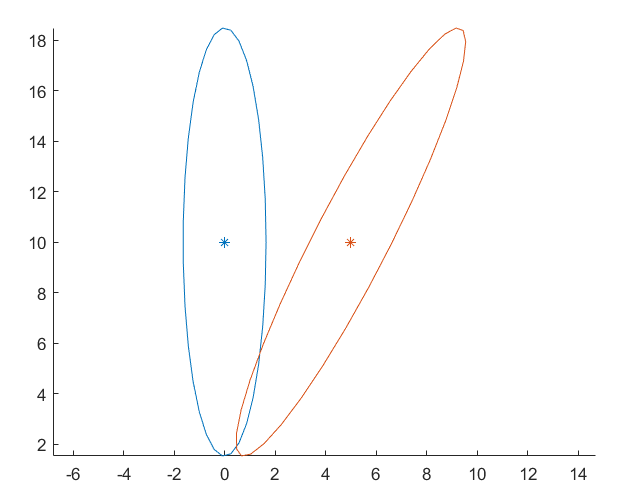
\includegraphics[width=0.7\textwidth]{images/picfor1c.png}
 \caption{Covariance of Z and q}
 \label{1c}
\end{figure}

\subsubsection{For mean}

The matrix A shifts the mean of q by a factor of 0.5 in the x-direction, resulting in a mean of z that is shifted by 5 in the x-direction and unchanged in the y-direction.

\subsubsection{For covariance}
The correlation coefficient of $ p $ is $ 0 $ , while after transformation it turns to 4/(sqrt(2.3)*sqrt(8))=0.9325. It is also shown in the picture that the axis of the ellipse leans an angle after transformation.

\subsubsection{Traced back}
According to the A matrix, this arises because the off-diagonal element of A reflects the fact that the x-component of z (z1) depends on both the x-component (q1) and the y-component (q2) of q. As a result, the transformation with A introduces a correlation between the individual components of z that was not present in q.


